\documentclass{amsart}
\usepackage{fullpage}
\usepackage{amsmath}
\usepackage{amsthm}
\usepackage{graphicx}
\DeclareGraphicsExtensions{.pdf,.png}
\newtheorem{thm}{Theorem}
\begin{document}
\title{Better Bound Simulations}
\author{Nelson Ray}
\maketitle
\section{Theory}
On page 151 of ``Normal Approximation by Stein's Method'', theorem 5.3
states
\begin{thm}
  If $W$, $W'$ is a variance one $\lambda$-Stein pair satisfying
  $|W'-W| \leq \delta$ then
  \begin{equation*}
    \sup_{z \in \mathbb{R}} |P(W \leq z) - P(Z \leq z)| \leq B + 
    \frac{.41\delta^3}{\lambda} + 1.5 \delta.
  \end{equation*}
\end{thm}

We need $\delta$ to be $O(N^{-1/2})$ in order for the total bound to
be of that order.  

We observe two samples with equal sample size: $S_1 = \{u_i\}_{i=1}^N$ and $S_2 =
\{u_i\}_{i=N+1}^{2N}$.  
Student's two-sample $t$-statistic is given by
\begin{align*}
T_{\Pi}(\{u_{\Pi(i)}\}_{i=1}^N, \{u_{\Pi(i)}\}_{i=N+1}^{2N}) 
&= \frac{\bar{u}_{1,\Pi} - \bar{u}_{2,\Pi}}{\sqrt{\frac{\frac{1}{N-1}
      \sum_{i=1}^N(u_{\Pi(i)} - \bar{u}_{1,\Pi})^2}{N} + \frac{\frac{1}{N-1}
      \sum_{i=N+1}^{2N}(u_{\Pi(i)} - \bar{u}_{2,\Pi})^2}{N}}} \\
\end{align*}

We need to set $\delta = \max_{\pi, i, j} |T_{\pi} - T_{\pi \circ (i, j)}|$ 
so that the bound is tight.  This appears to be a daunting
optimization problem.  There are $(2N)!$ permutations and $N^2$
possible transpositions $(i, j)$ for each permutation.  Well, because the
$t$-statistic is invariant to permutations within groups, there are
$\binom{2N}{N}$ (really, $\binom{2N}{N} / 2$ because of symmetry)
permutations to consider.  And there are probably some tricks we can
apply to reduce the $N^2$.  But this still doesn't seem to be very
tractable.

\section{$T$ and $T'$}
Let's first plot all possible values of $T$, and the corresponding
value of $T'$ that maximizes $|T-T'|$.  Here, we make $N$ draws of
sample 1 from $\mathcal{N}(\mu, 1)$ and $N$ draws of sample 2 from
$\mathcal{N}(0, 1)$, varying $N \in \{5, 6, 7\}$ and $\mu \in \{1, 2,
5\}$, coloring the $(T, T')$ pair that maximizes $|T-T'|$.  There is
some symmetry (the pair shows up 4 times) because of swapping $T$ with
$-T$ (2 swaps) and $T'$ with $T$ (2 swaps).

\begin{figure}[!ht]
  \centering
  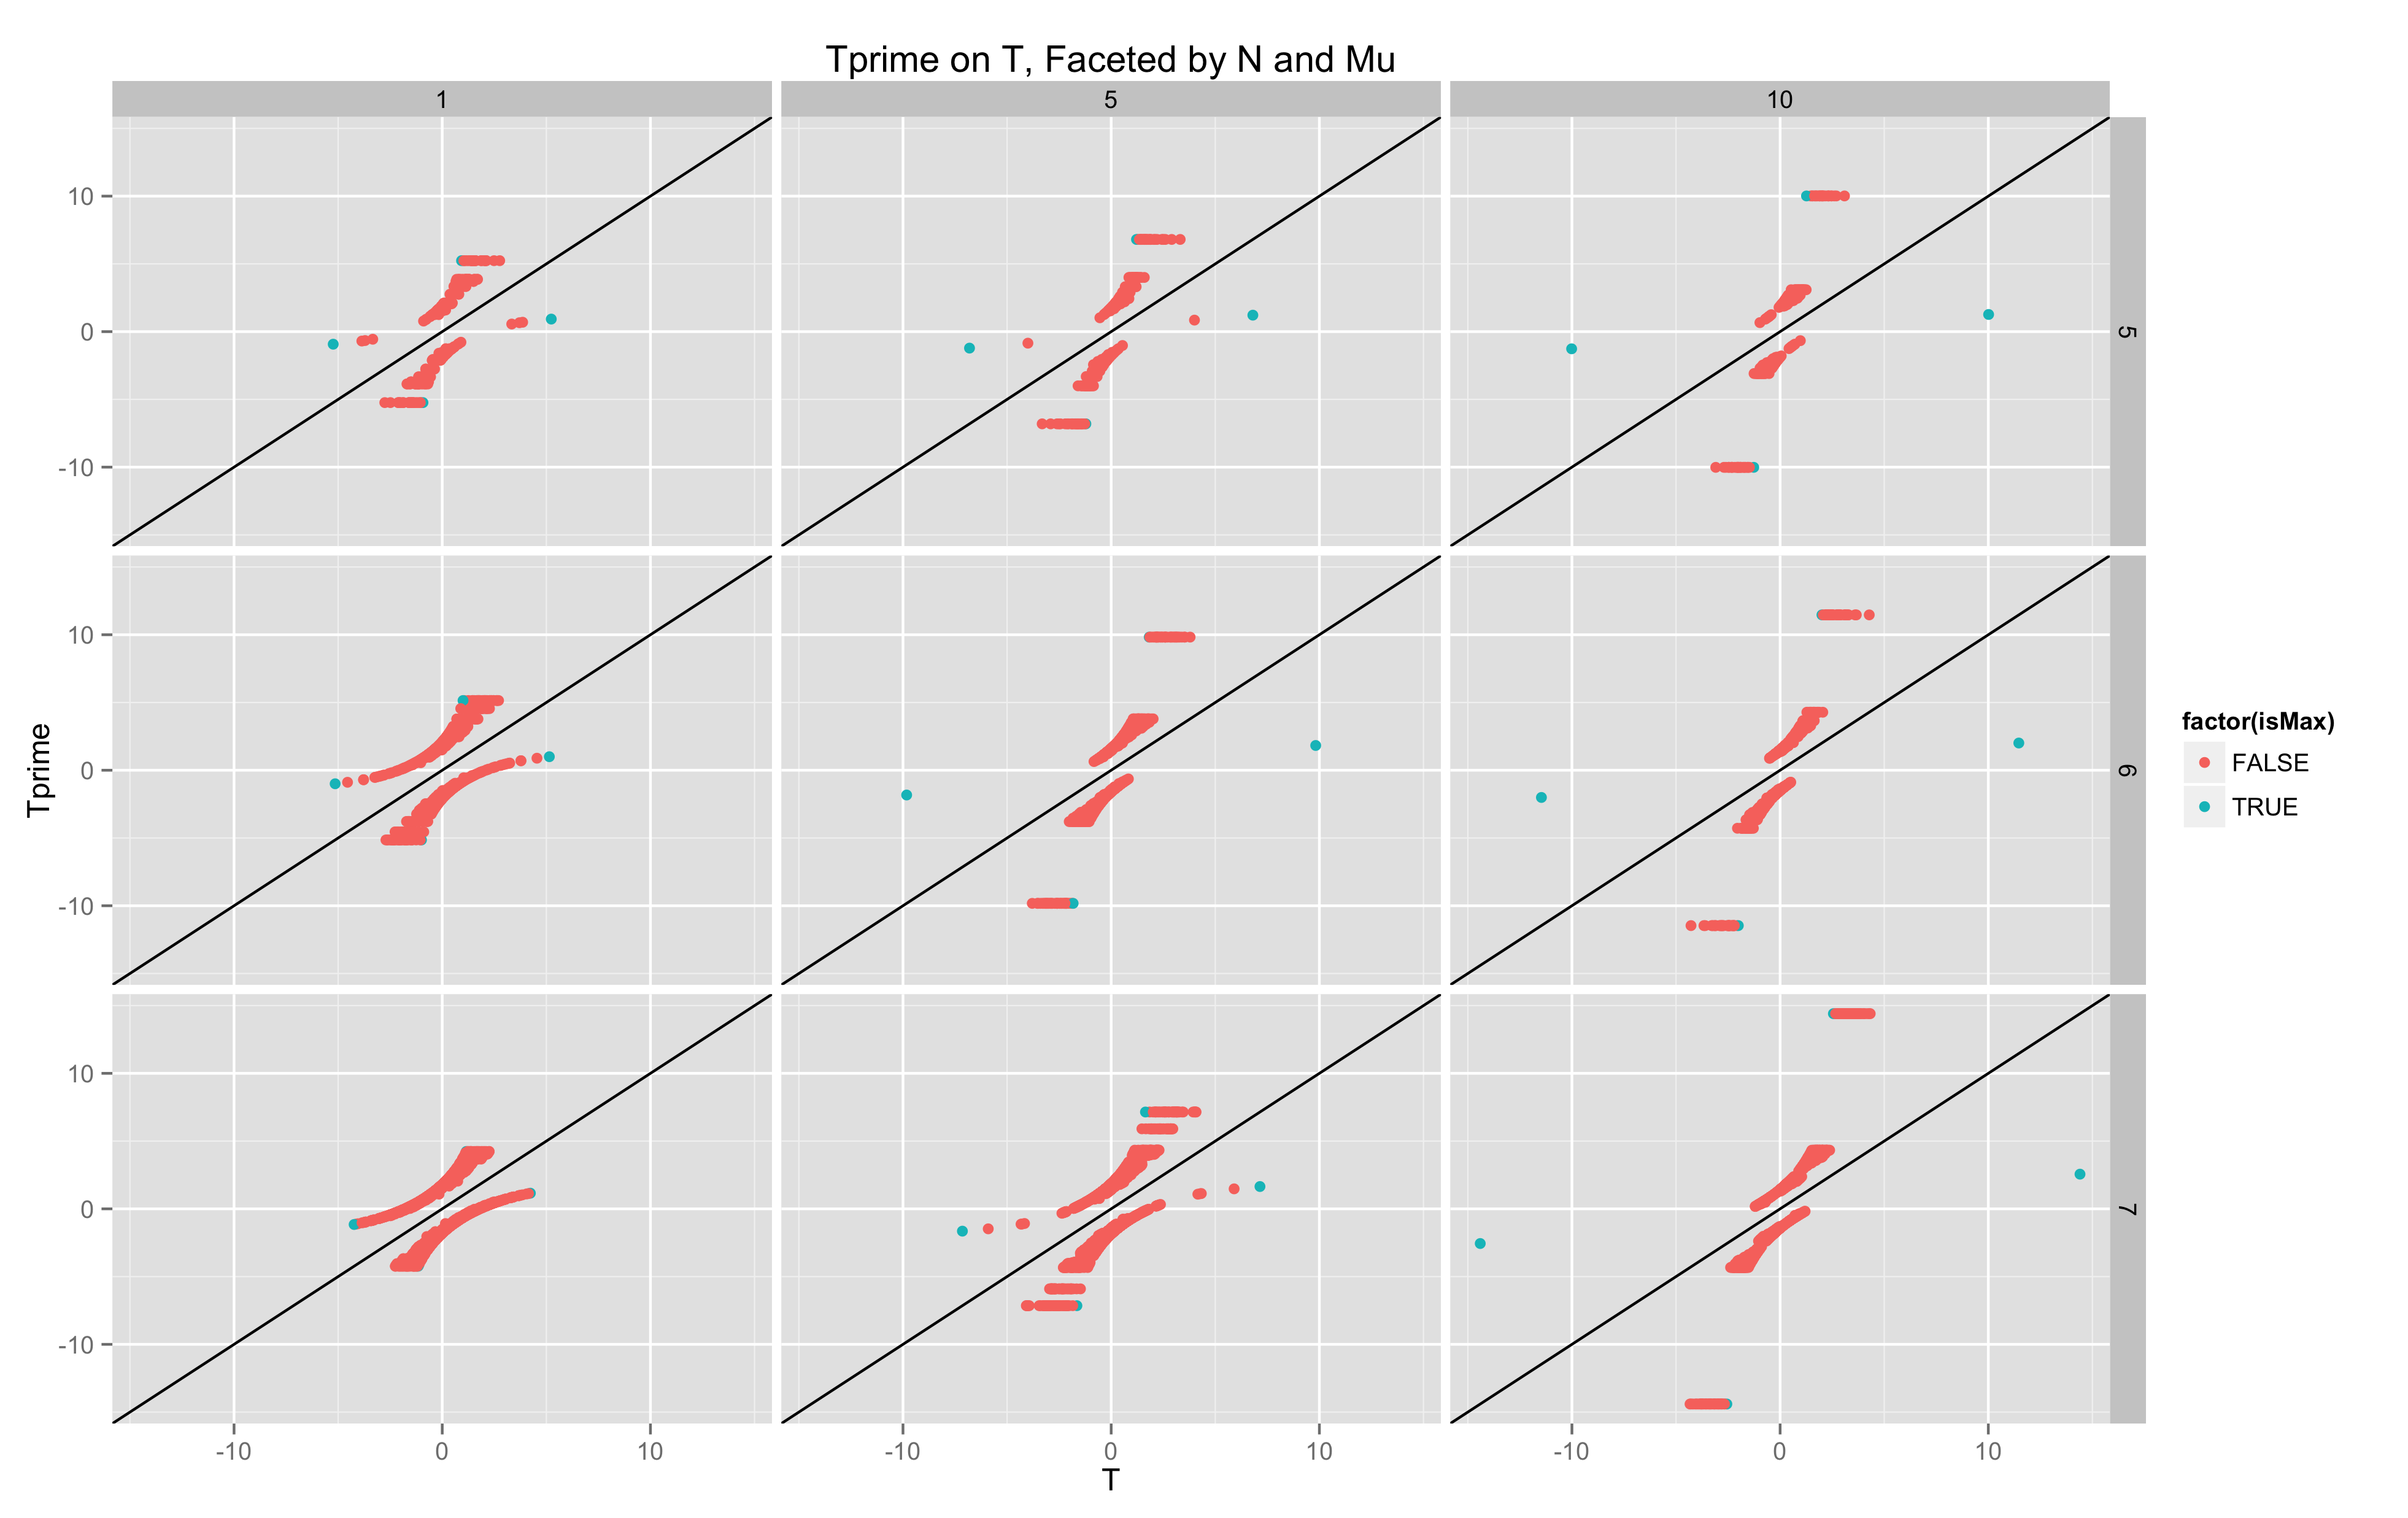
\includegraphics[scale=.12]{t_tprime_plot.png}
\end{figure}

Unfortunately, we can't make $N$ much bigger than 7 using the current
technique.  
\clearpage

\section{Shortcut}
It always seems to be the case that, say, the minimum (equivalently,
the maximum due to symmetry) value of $T_{\pi}$ maximizes $|T - T'|$.
Knowing the permutation $\pi$ that maximizes $|T - T'|$, we can try to
figure out the corresponding transposition $(i, j)$.  

It seems reasonable that sorting the data into its order statistics
$\{u_{(i)}\}_{i=1}^{2N}$ will minimize $T$.  That is, let the $N$
smallest be in the first group and the next $N$ in the second.  

Another thing that seems reasonable to find the $(i, j)$ that maximizes
$|T - T'|$ is to swap the ``most different'' sample of the first group
with that of the second group: $u_{(1)}$ with $u_{(2N)}$.

I tried this shortcut (it only really involves sorting the data) and
compared it with the exact methodology of the above section and found
agreement in all the tested settings.  This lets us really ramp up $N$
in our simulations.

I haven't really tried to prove it yet: it looks challenging.

Consider drawing sample 1 from $\mathcal{N}(2, \sigma^2)$ and sample 2
from $\mathcal{N}(0, \sigma^2)$ where $\sigma = 1$:
\begin{figure}[!ht]
  \centering
  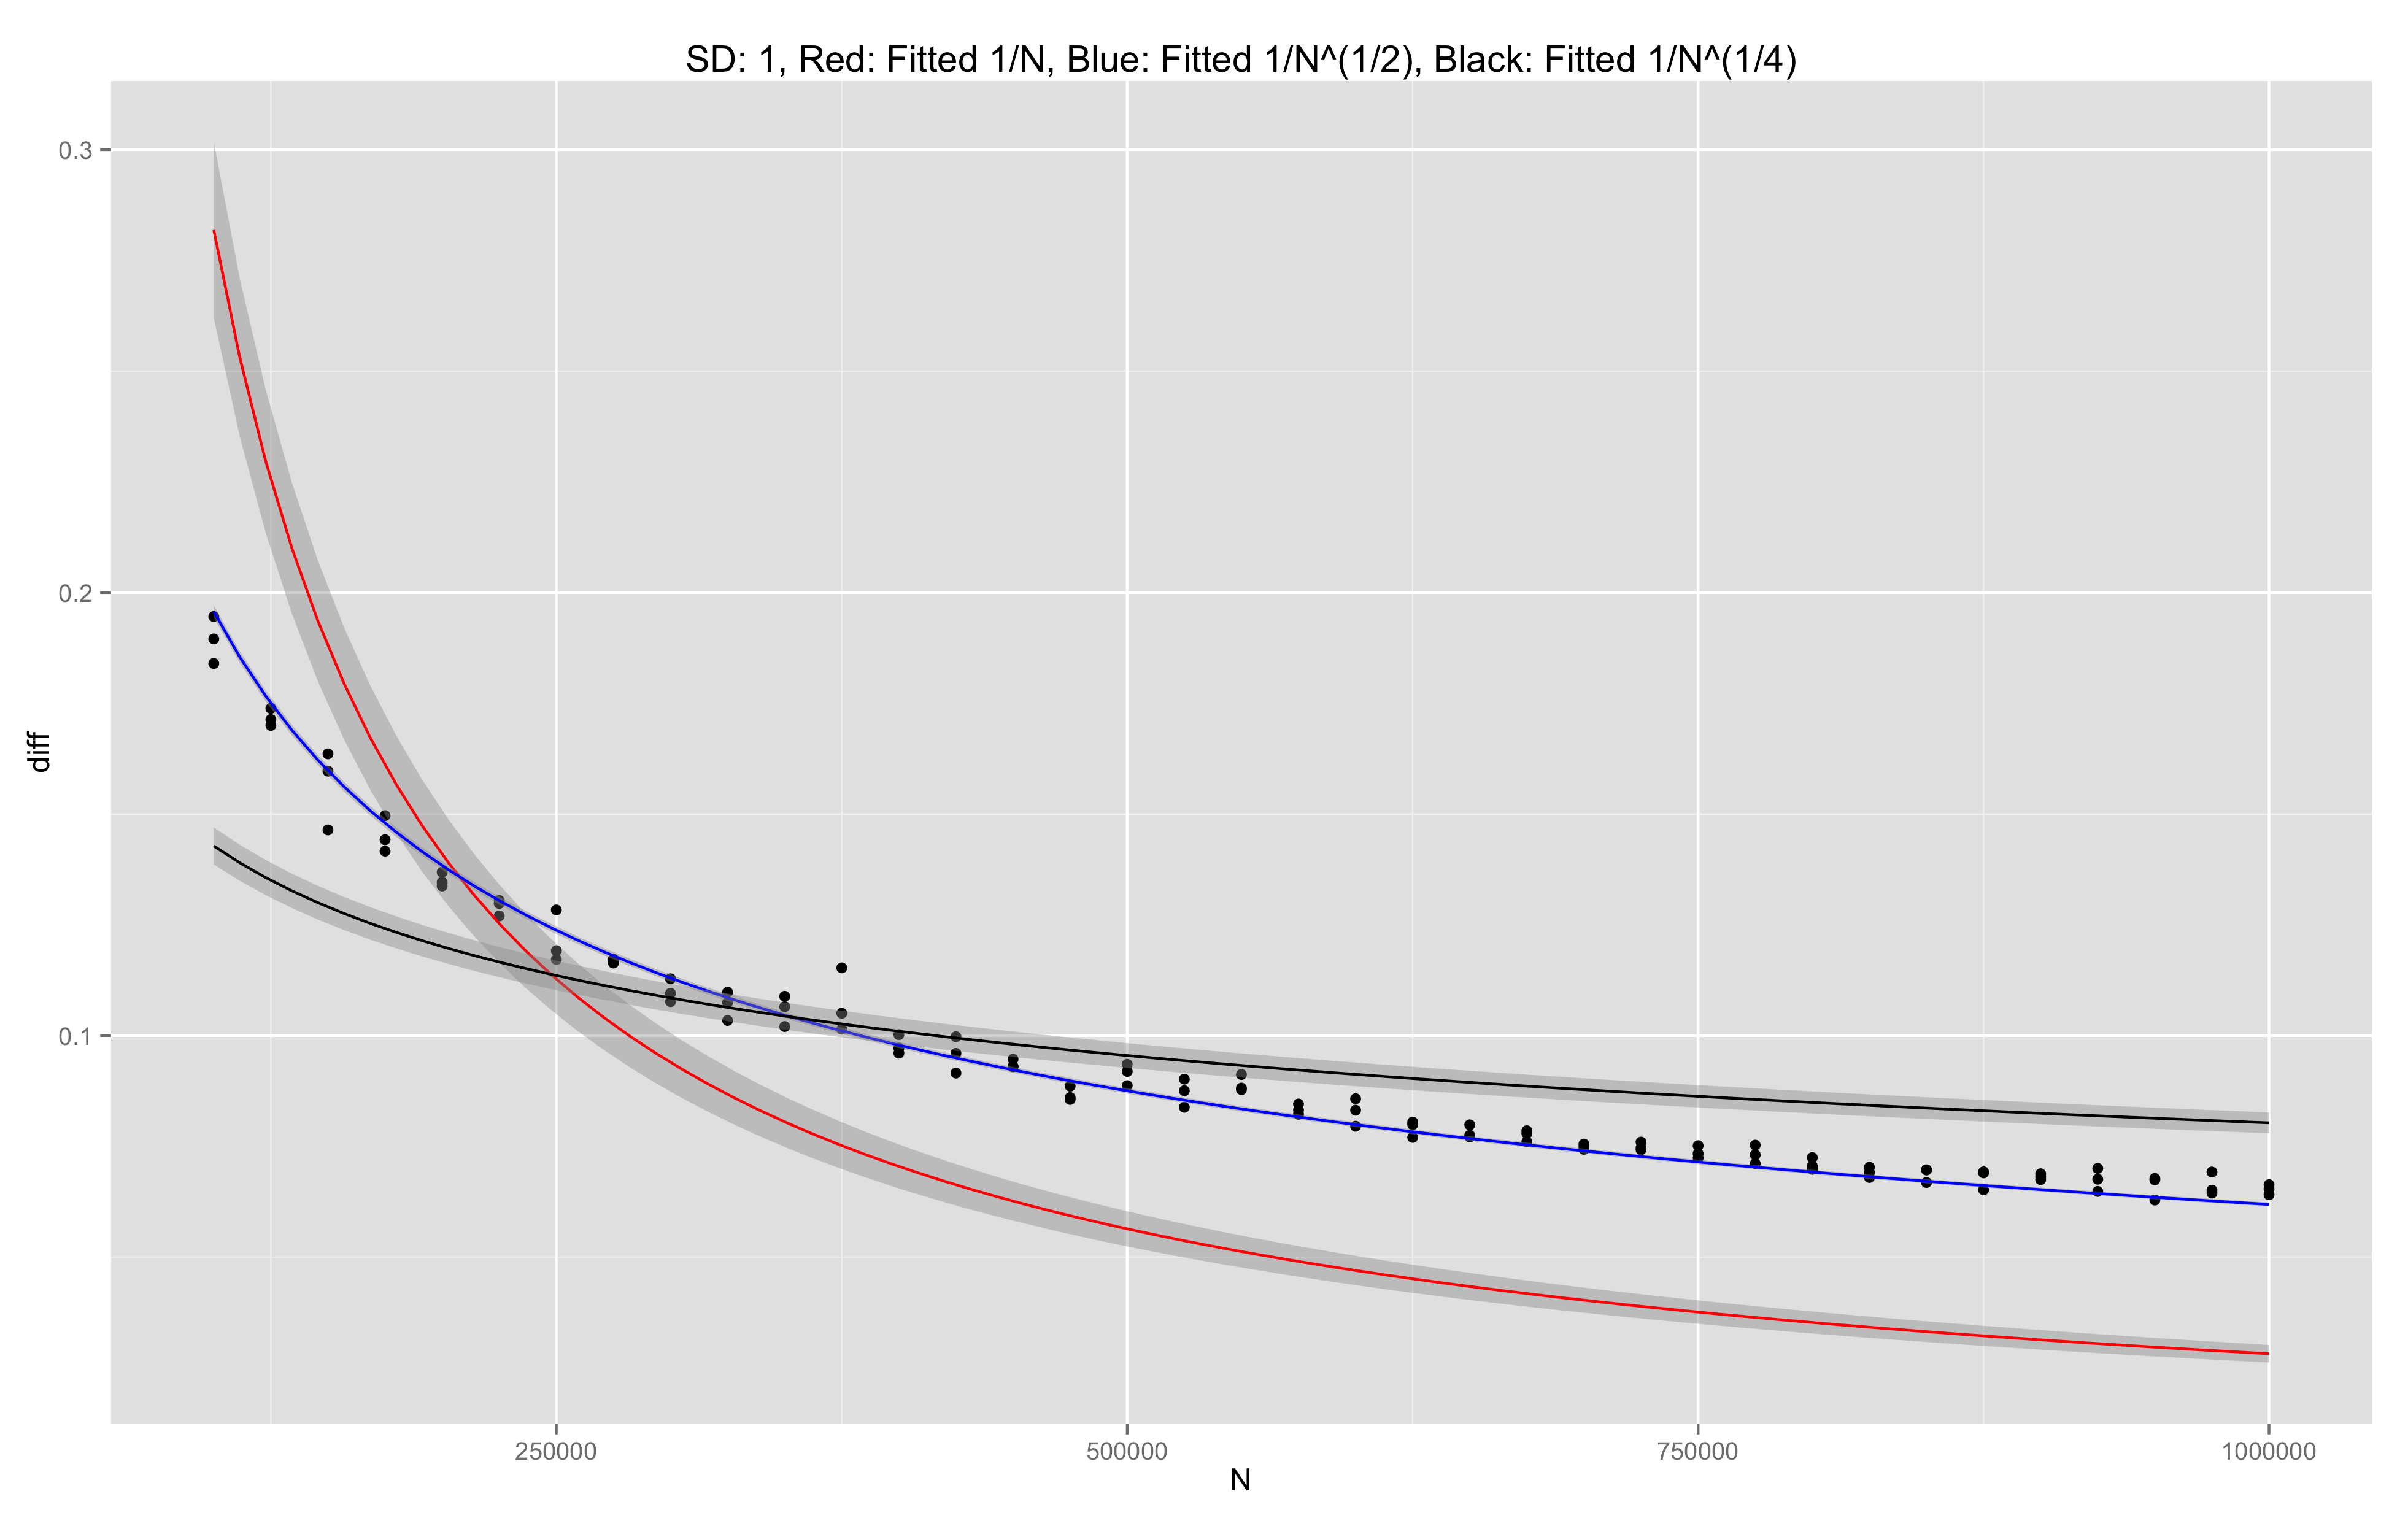
\includegraphics[scale=.06]{rate_plot_1.png}
\end{figure}

Now consider $\sigma = \sqrt{N}$ (so the power is constant in the
sample size):
\begin{figure}[!ht]
  \centering
  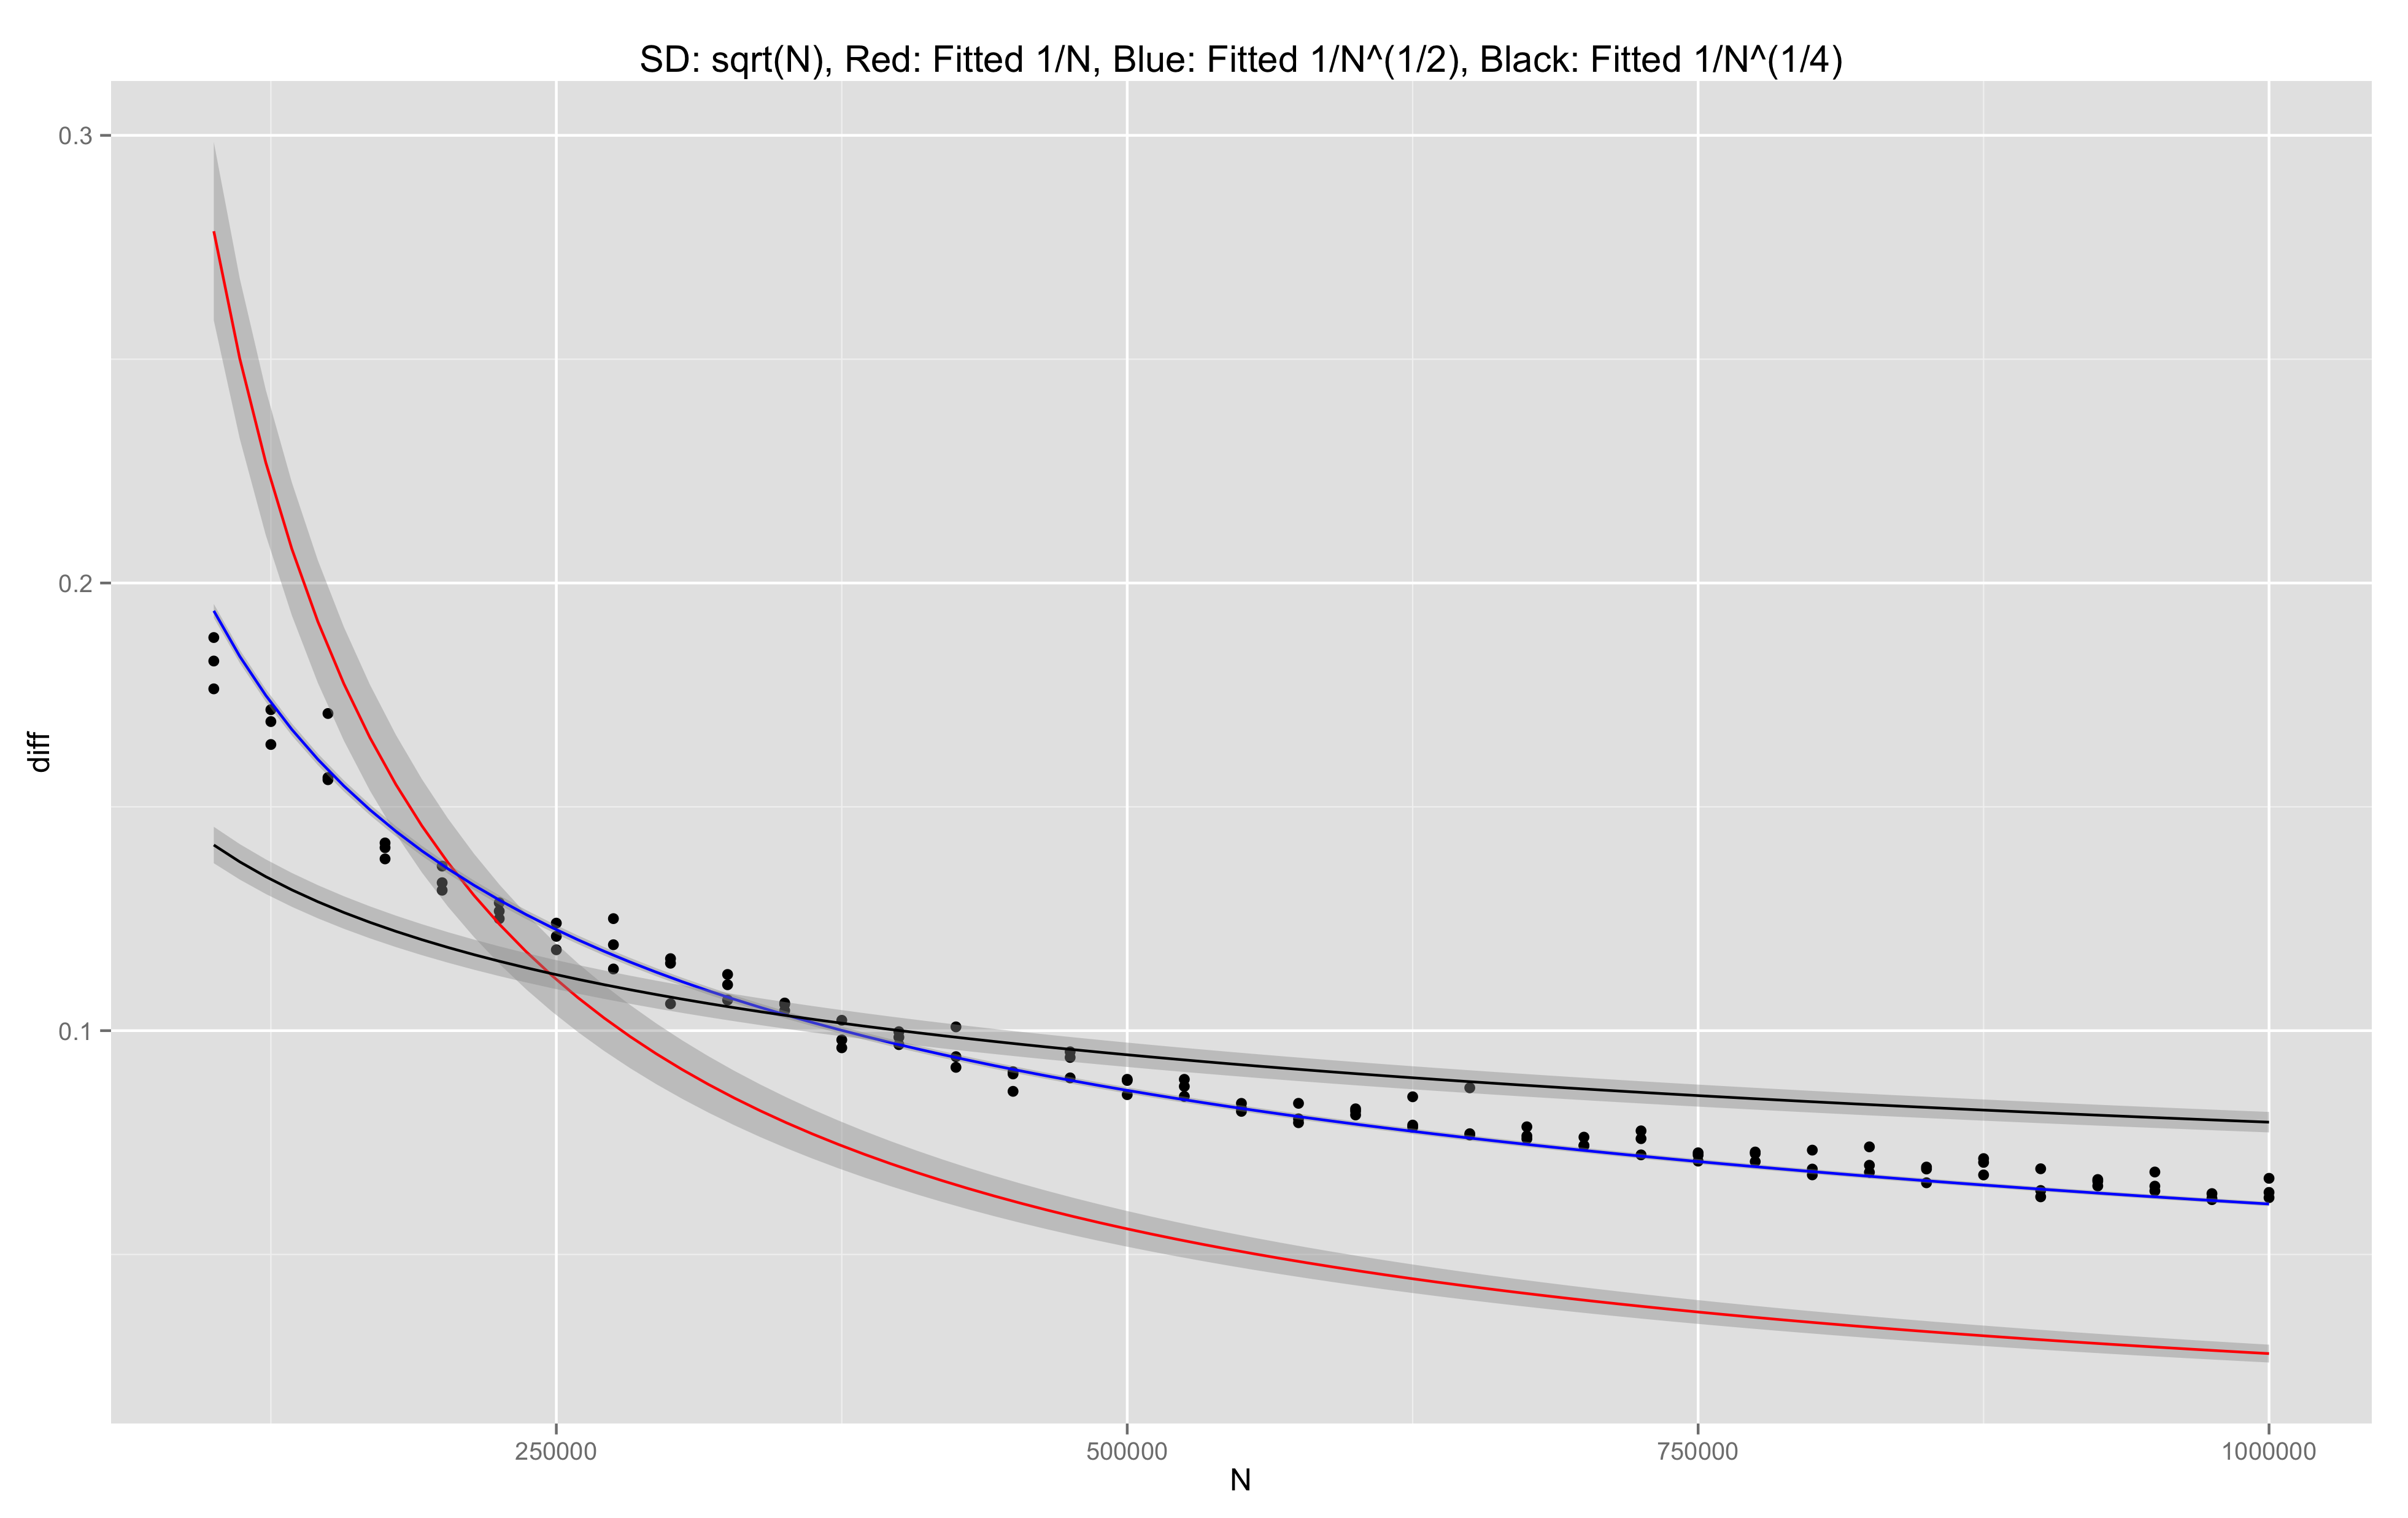
\includegraphics[scale=.06]{rate_plot_2.png}
\end{figure}

Finally, $\sigma = \frac{1}{\sqrt{N}}$:
\begin{figure}[!ht]
  \centering
  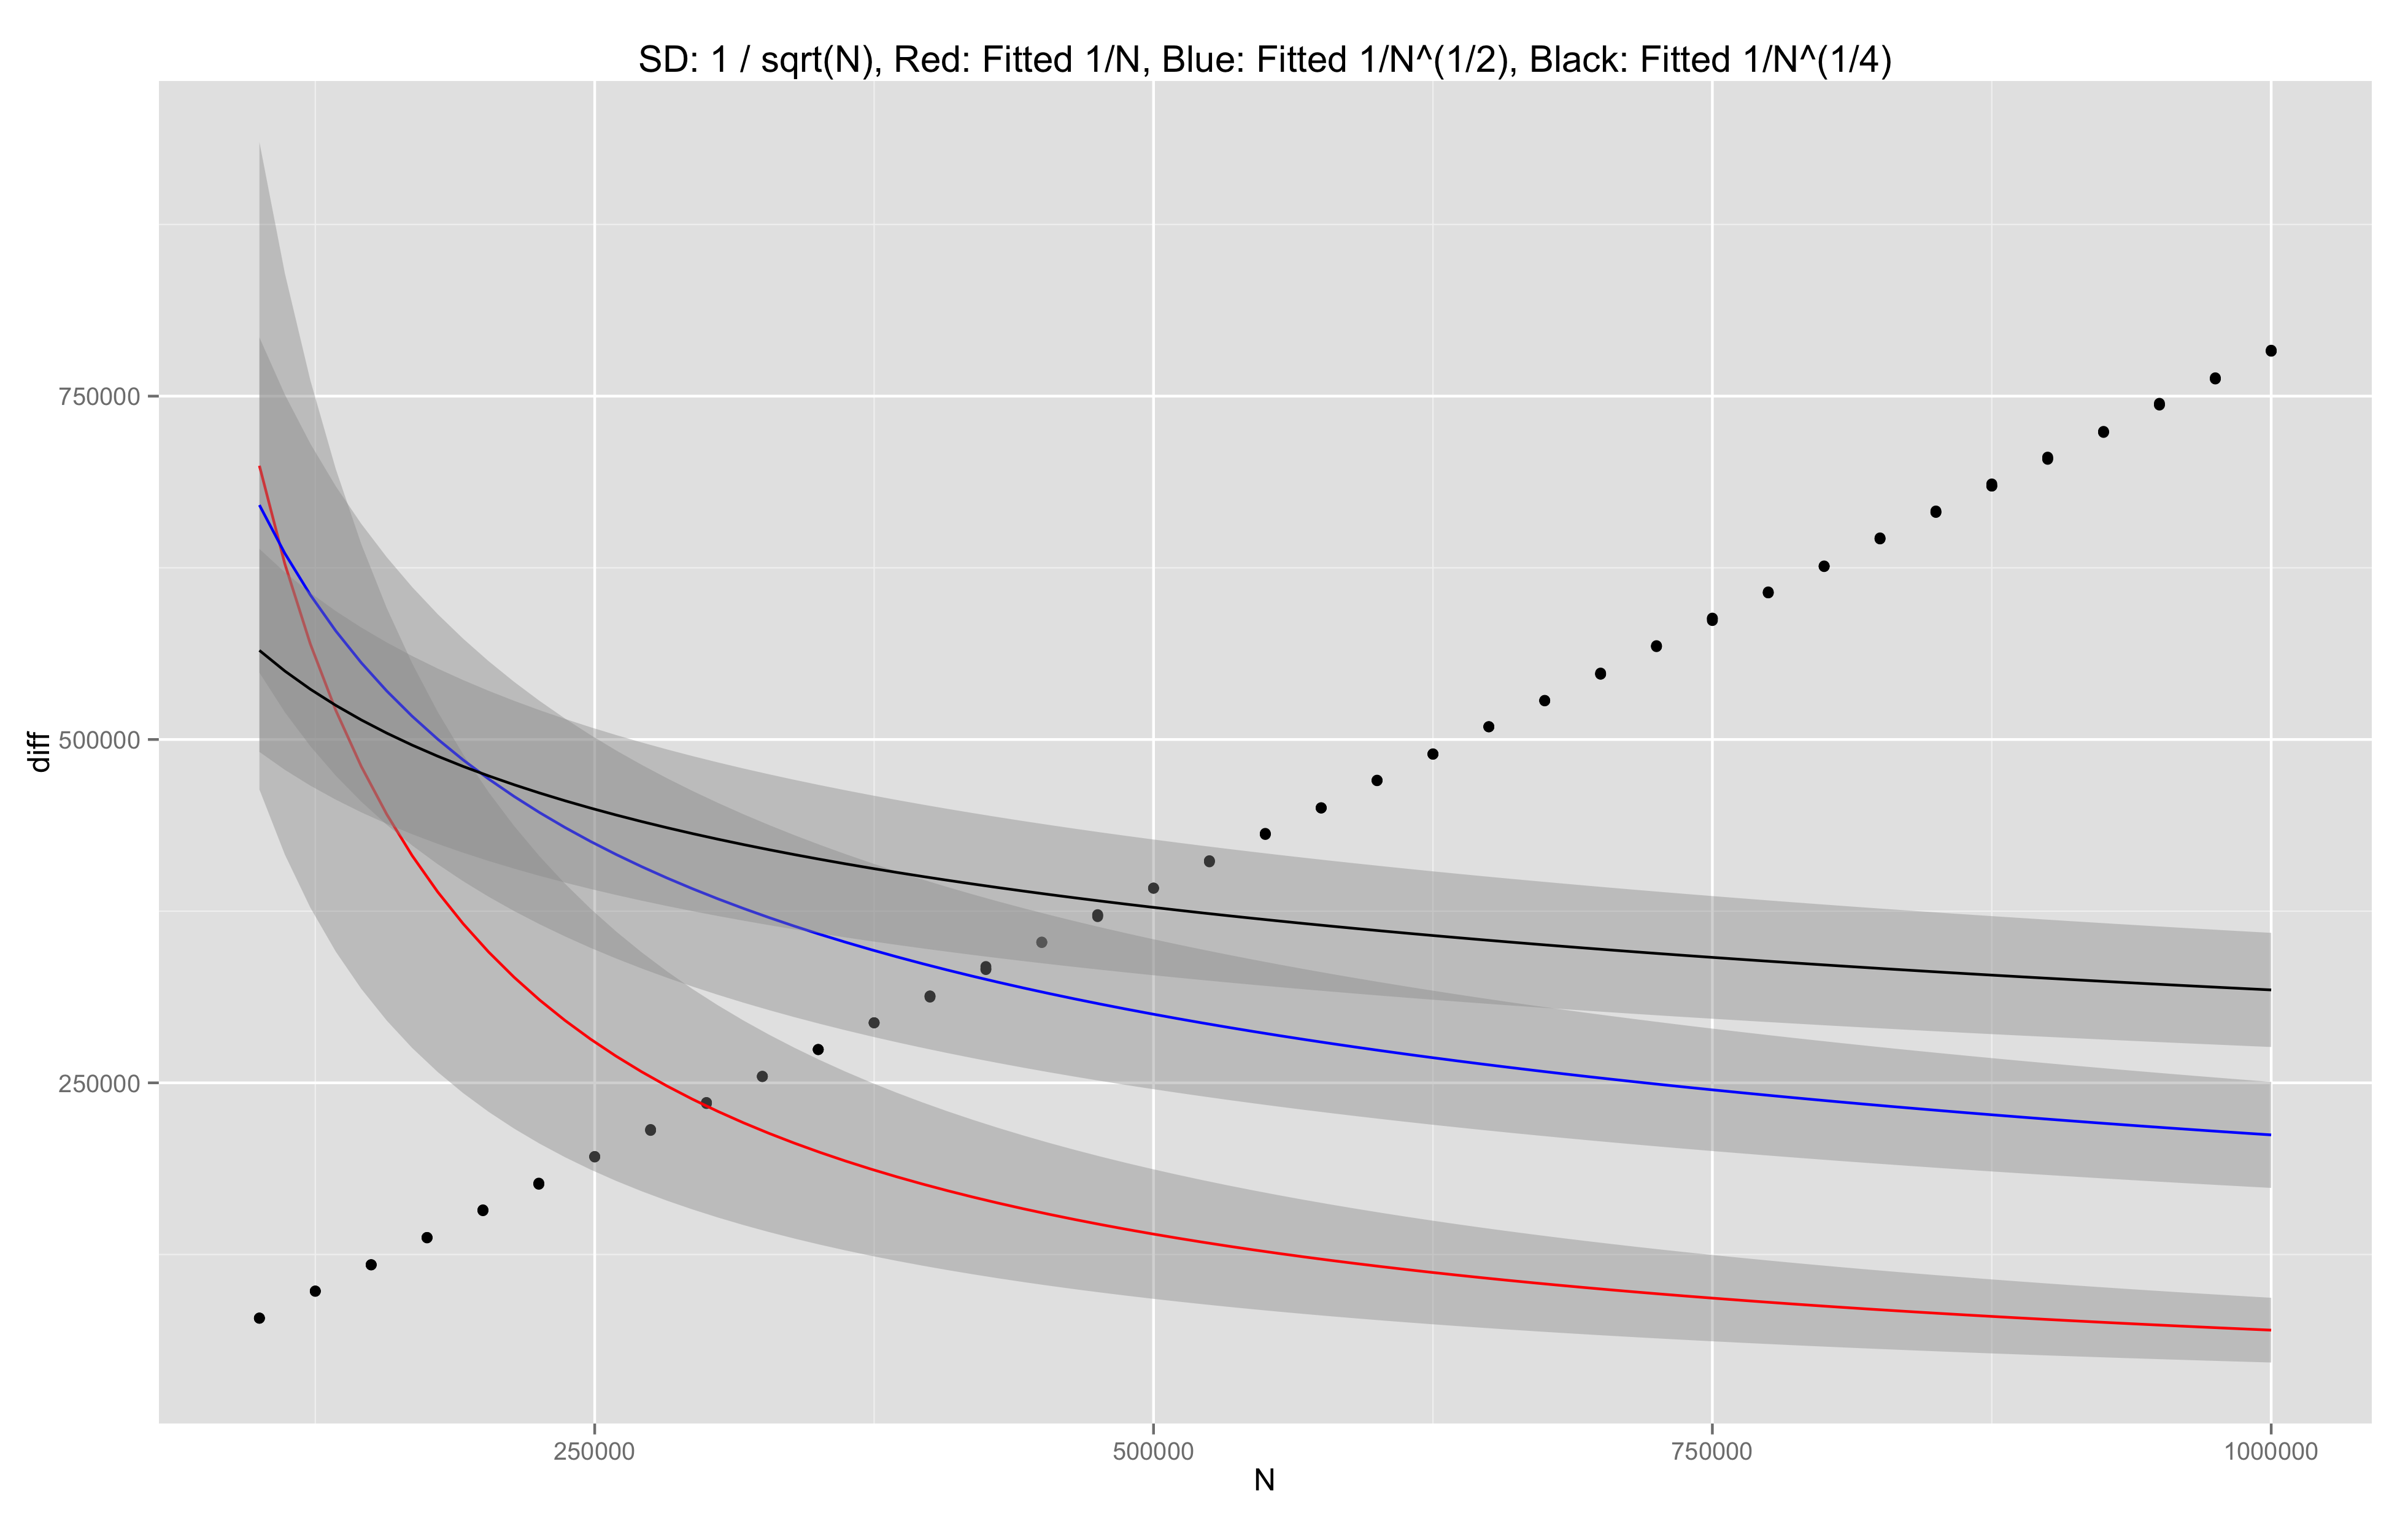
\includegraphics[scale=.06]{rate_plot_3.png}
\end{figure}

The last situation is one of those pathological cases that we were
trying to avoid, where the within-group variance vanishes so the
distributions tend toward point masses.  But the other reasonable
cases look good.  That is, if the shortcut works, it appears that 
$\delta = \max_{\pi, i, j} |T_{\pi} - T_{\pi \circ (i, j)}|$ is
$O(N^{-1/2})$ for these reasonable cases.
\end{document}
